\section{Results}
\label{sec:results}

% \mc{Result tables: you can write results as e.g., 35.8 rather than 0.358}



We begin by maximizing single-LLM performance (\S \ref{sec:single_model}). Next, we assess the potential of multi-LLM collaboration through oracle model selection (\S \ref{sec:oracle}), before exploring the benefits of debate alone (\S \ref{sec:debate_only}) and in combination with self-reflection (\S \ref{sec:selfreflect_debate}).


\definecolor{lightgray}{gray}{0.9}
\definecolor{highgreen}{rgb}{0.1608, 0.5804, 0.2196}
\definecolor{lowred}{rgb}{0.9216, 0.1569, 0.1569}


\begin{table}[!htp]
\centering
\resizebox{\linewidth}{!}{%
    \begin{tabular}{l l l l l l}
    \specialrule{1.3pt}{0pt}{0pt}
    \textbf{Label/Model} & \textbf{Si (w/o)} & \textbf{Si (w/)} & \textbf{Self-Reflect} \\
    \toprule

    \textsc{Yes-Only} & 35.8 & - & - \\
    \textsc{No-Only} & 33.2 & - & - \\
    \textsc{Neither-Only} & 31.0 & - & - \\
    \midrule

    \textsc{LLaMA-3} & 49.5 & 63.7 \scriptsize{\textcolor{highgreen}{(+28.7)}} & \textbf{65.7} \scriptsize{\textcolor{highgreen}{(+3.14)}} \\
    
    \textsc{Gemma-2} & 50.7 & 68.9 \scriptsize{\textcolor{highgreen}{(+35.9)}} & \textbf{72.5} \scriptsize{\textcolor{highgreen}{(+5.22)}} \\
    % \midrule


    \textsc{EXAONE-3} & 42.8 & 63.5 \scriptsize{\textcolor{highgreen}{(+48.4)}} & \textbf{64.3} \scriptsize{\textcolor{highgreen}{(+1.26)}} \\
    
    \textsc{Yi-1.5} & 51.0 & 70.7 \scriptsize{\textcolor{highgreen}{(+38.6)}} & \textbf{71.5} \scriptsize{\textcolor{highgreen}{(+1.13)}} \\
    
    \textsc{InternLM-2.5} & 47.0 & 67.8 \scriptsize{\textcolor{highgreen}{(+44.3)}} & \textbf{70.7} \scriptsize{\textcolor{highgreen}{(+4.28)}} \\ 
    % \midrule



    \textsc{Aya-23} & 49.4 & 65.8 \scriptsize{\textcolor{highgreen}{(+33.2)}} & \textbf{68.1} \scriptsize{\textcolor{highgreen}{(+3.50)}} \\
    
    \textsc{SeaLLM-3} & 49.5 & 68.1 \scriptsize{\textcolor{highgreen}{(+37.6)}} & \textbf{69.3} \scriptsize{\textcolor{highgreen}{(+1.76)}} \\

    \rowcolor{lightgray} \textit{\textsc{Gemma-2-27b}} & 55.8 & 79.2 \scriptsize{\textcolor{highgreen}{(+41.9)}} & \textbf{80.1} \scriptsize{\textcolor{highgreen}{(+1.14)}} \\


    \specialrule{1.3pt}{0pt}{0pt}
    \end{tabular}
}
\caption{Mean accuracies (\%) for Single Model and Self-Reflection baselines. \textbf{Si (w/o):} Single Model without rule-of-thumb information; \textbf{Si (w/):} Single Model with rule-of-thumb information; \textbf{Self-Reflect:} Self-Reflection. Best scores for each row are in \textbf{bold}. \textcolor{highgreen}{Green} text is the \% of improvements compared to the adjacent left column. We include accuracies for \fcolorbox{white}{lightgray}{\textsc{Gemma-2-27b}} judge LLM as reference. Fine-grained results for each country are detailed in Appendix \ref{appendix:detailed_single_llm}.}
\label{tab:single_llm_new}
\end{table}


\subsection{Self-Reflection Improves Single-LLM Accuracy}
\label{sec:single_model}

We empirically investigate the impact of contextualization and multi-turn interactions on a single LLM. For cultural contextualization, we adopt the most effective method from \textsc{NormAd-eti} \cite{normad}: including a social norm relevant to the story (\textit{rule-of-thumb}) in the prompt. As shown in Table \ref{tab:single_llm_new} (\textbf{Si w/}), this method consistently improves mean accuracies by up to 48.4\% and 39.1\% on average across all tested LLMs. This confirms the previous findings that adding relevant cultural context can significantly enhance cultural alignment of LLMs \cite{zhu-etal-2024-large, normad}. Accordingly, we include the rule-of-thumb information in the prompts for all subsequent experiments.



Next, we find that single LLMs can generate feedback on their own outputs and reflect upon it, resulting in an average accuracy improvement of 3.26\% across all tested LLMs through self-reflection. In Table \ref{tab:single_llm_new}, the rankings of \textbf{Si (w/o)} and \textbf{Si (w/)} are strongly positively correlated ($r$=0.85), as well as \textbf{Si (w/)} and \textbf{Self-Reflect} ($r$=0.95), which indicates that stronger base LLMs generally benefit more from both cultural contextualization and self-reflection. 
% \zk{Add citation that stronger base llms can use the context/self-reflect better than weaker ones}
% optimized internal representations, making them less reliant on iterative feedback loops for improvement compared to weaker LLMs.

%We select LLMs distinct from those tested in 
While prior models evaluated on the \textsc{NormAd-Eti} dataset were English-centric\footnote{This includes \textsc{LLaMA-1}, \textsc{LLaMA-2}, \textsc{Mistral-3}, \textsc{Olmo}, \textsc{GPT-3.5-turbo}, and \textsc{GPT-4}.} \cite{normad}, our experiments consider a more diverse range of LLMs, which outperform the prior best-performing variant (\textsc{Mistral-7b-instruct} \cite{mistral} with rule-of-thumb information, which achieved a mean accuracy of 40.7\%). 

% \mc{How do the set of models tested here differ or overlap with those tested in the Normad paper? In terms of raw performance how do these results compare with those from the Normad paper?}

% \zk{Their best model is using single Mistral-7b model with ROT which has precision as 0.82 (recall 0.81 and F1 score as 0.81), if we convert to accuracy using precision and recall, it becomes 0.407.}

\definecolor{lightgray}{gray}{0.9}
\definecolor{highgreen}{rgb}{0.1608, 0.5804, 0.2196}
\definecolor{lowred}{rgb}{0.9216, 0.1569, 0.1569}

% orange, green, purple
\definecolor{orange}{rgb}{1, 0.6392, 0.2784}
\definecolor{green}{rgb}{0.3255, 0.6706, 0.2}
\definecolor{purple}{rgb}{0.6118, 0.3569, 0.8706}
\definecolor{highlightgreen}{rgb}{0.6, 0.9, 0.7}
\definecolor{lightgreen}{RGB}{229, 247, 195}
\definecolor{rred}{RGB}{201, 69, 64}


\begin{table*}[!htp]
\centering
\resizebox{\linewidth}{!}{%
    \begin{tabular}{lllllllllll}
    \specialrule{1.3pt}{0pt}{0pt}
    \textbf{$\mathcal{M}_1$} & \textbf{$\mathcal{M}_2$} & \textbf{Si($\mathcal{M}_1$)} & \textbf{Si($\mathcal{M}_2$)} & \textbf{\textcolor{orange}{Ora}} & \textbf{\textcolor{rred}{D($\mathcal{M}_1$)}} & \textbf{\textcolor{rred}{D($\mathcal{M}_2$)}} & \textbf{\textcolor{rred}{D}} & \textbf{\textcolor{purple}{S+D($\mathcal{M}_1$)}} & \textbf{\textcolor{purple}{S+D($\mathcal{M}_2$)}} & \textbf{\textcolor{purple}{S+D}} \\
    \toprule
% \textbf{804*\dag}
    \multirow{6}{*}{\textsc{LLaMA-3}} & \textsc{Gemma-2} & \multirow{6}{*}{63.7} & 68.9 & 82.6 & \underline{66.5} & \underline{76.7} & \cellcolor{lightgreen}{\bfseries 79.7*\dag} & \underline{69.2} & 63.4 & 75.9* \\
    
    & \textsc{EXAONE-3} & & 63.5 & 87.5 & \underline{70.7} & 63.5 & 75.4* & \underline{72.2} & \underline{64.5} & \textbf{78.2*\dag} \\
    
    & \textsc{Yi-1.5} & & 70.7 & 77.3 & \underline{66.0} & \underline{\textbf{76.6}} & 74.7 & \underline{68.2} & \underline{75.7} & 74.5 \\
    
    & \textsc{InternLM-2.5} & & 67.8 & 74.8 & \underline{65.3} & \underline{73.8} & 74.7* & \underline{70.5} & 36.9 & \textbf{74.8*\dag} \\
    
    & \textsc{Aya-23} & & 65.8 & 72.9 & \underline{67.8} & \underline{\textbf{77.5}} & 77.0 & \underline{68.1} & \underline{77.3} & 73.8 \\
    
    & \textsc{SeaLLM-3} & & 68.1 & 82.4 & 63.7 & \underline{76.6} & 75.7 & \underline{67.6} & \underline{\textbf{78.6}} & 74.7 \\
    \midrule

    \multirow{5}{*}{\textsc{Gemma-2}} & \textsc{EXAONE-3} & \multirow{5}{*}{68.9} & 63.5 & 82.3 & \underline{77.7} & \underline{64.8} & 78.6* & \underline{79.6} & \underline{65.5} & \cellcolor{lightgreen}{\bfseries 80.4*\dag} \\
    
    & \textsc{Yi-1.5} & & 70.7 & 83.3 & \underline{75.6} & \underline{77.1} & \textbf{78.5*} & \underline{76.0} & \underline{73.9} & 77.6* \\
    
    & \textsc{InternLM-2.5} & & 67.8 & 82.8 & \underline{77.1} & \underline{73.2} & \textbf{78.5*} & \underline{75.8} & 28.3 & 77.7* \\
    
    & \textsc{Aya-23} & & 65.8 & 82.6 & \underline{71.3} & \underline{76.3} & \cellcolor{lightgreen}{\bfseries 79.7*} & 64.6 & \underline{75.8} & 76.0 \\
    
    & \textsc{SeaLLM-3} & & 68.1 & 83.8 & \underline{75.8} & \underline{78.2} & \textbf{79.0} & \underline{74.9} & \underline{78.5} & 78.6 \\
    \midrule

    \multirow{4}{*}{\textsc{EXAONE-3}} & \textsc{Yi-1.5} & \multirow{4}{*}{63.5} & 70.7 & 90.8 & \underline{64.5} & \underline{77.6} & 75.5 & \underline{65.7} & \underline{76.3} & \textbf{77.7*\dag} \\
    
    & \textsc{InternLM-2.5} & & 67.8 & 91.3 & \underline{66.1} & \underline{77.3} & \textbf{78.5*} & \underline{66.1} & 48.7 & 70.9* \\
    
    & \textsc{Aya-23} & & 65.8 & 91.6 & \underline{65.2} & \underline{76.9} & 77.5 & \underline{65.4} & \underline{77.2} & \textbf{78.5*\dag} \\
    
    & \textsc{SeaLLM-3} & & 68.1 & 82.8 & \underline{64.9} & \underline{\textbf{79.5}} & 77.6 & \underline{65.5} & \underline{79.4} & 79.3 \\
    \midrule

    \multirow{3}{*}{\textsc{Yi-1.5}} & \textsc{InternLM-2.5} & \multirow{3}{*}{70.7} & 67.8 & 75.7 & \underline{74.1} & \underline{70.1} & 73.9 & \underline{73.2} & 40.3 & \textbf{74.4*\dag} \\
    
    & \textsc{Aya-23} & & 65.8 & 74.1 & 54.8 & \underline{67.3} & 69.9* & \underline{72.5} & \underline{71.5} & \textbf{72.8\dag} \\
    
    & \textsc{SeaLLM-3} & & 68.1 & 83.9 & \underline{72.7} & \underline{74.4} & 74.0 & \underline{71.7} & \underline{\textbf{74.9}} & 74.1\dag \\
    \midrule

    \multirow{2}{*}{\textsc{InternLM-2.5}} & \textsc{Aya-23} & \multirow{2}{*}{67.8} & 65.8 & 70.8 & \underline{71.0} & \underline{73.0} & 74.1* & \underline{70.8} & \underline{\textbf{73.3}} & 72.6 \\
    
    & \textsc{SeaLLM-3} & & 68.1 & 83.2 & \underline{70.2} & \underline{\textbf{76.3}} & 75.0 & \underline{70.1} & \underline{75.8} & 74.7 \\
    \midrule

    \textsc{Aya-23} & \textsc{SeaLLM-3} & 65.8 & 68.1 & 82.5 & \underline{71.0} & \underline{71.1} & \textbf{74.4*} & \underline{69.3} & \underline{69.7} & 70.1 \\
    \specialrule{1.3pt}{0pt}{0pt}

    \textbf{Average} & & 66.4 & 67.5 & 81.9 & \underline{69.1} & \underline{74.2} & \textbf{76.3*} & \underline{70.3} & \underline{66.9} & 75.6* \\

    \specialrule{1.3pt}{0pt}{0pt}
    \end{tabular}
}
\caption{Mean accuracies (\%) for Oracle model selection and Multi-Agent Debate baselines. Note that $\mathcal{M}_1$ and $\mathcal{M}_2$ are exchangeable thus the order does not matter. \textbf{Si($\mathcal{M}_i$):} Individual single model accuracies (with rule-of-thumb information) from Table \ref{tab:single_llm_new}; \textbf{\textcolor{orange}{Ora}:} Oracle model selection; \textbf{\textcolor{rred}{D($\mathcal{M}_i$)}, \textcolor{rred}{D}:} Individual and final accuracies in Debate-Only; \textbf{\textcolor{purple}{S+D($\mathcal{M}_i$)}, \textcolor{purple}{S+D}:} Individual and final accuracies in Self-Reflect+Debate. \textbf{Si($\mathcal{M}_i$)} $<$ \textbf{\textcolor{rred}{D($\mathcal{M}_i$)}} or \textbf{\textcolor{purple}{S+D($\mathcal{M}_i$)}} is \underline{underlined}.
\textbf{\textcolor{rred}{D($\mathcal{M}_i$)}} $<$ \textbf{\textcolor{rred}{D}} or \textbf{\textcolor{purple}{S+D($\mathcal{M}_i$)}} $<$ \textbf{\textcolor{purple}{S+D}} is marked as \textbf{*}. \textbf{\textcolor{rred}{D}} $<$ \textbf{\textcolor{purple}{S+D}} is marked as \dag.
Best scores for each row excluding \textbf{\textcolor{orange}{Ora}} are \textbf{bold}. \textbf{\textcolor{rred}{D}} or \textbf{\textcolor{purple}{S+D}} matching the judge LLM's single model accuracy (79.2\%) is highlighted \fcolorbox{white}{lightgreen}{light green}. All improvements are statistically significant ($p < 0.05$).}
\label{tab:multi_llm}
\end{table*}

% Absolute best score is highlighted \fcolorbox{white}{highlightgreen}{green}.


\subsection{Distinct LLMs are Complementary}% can \textit{complement} their cultural knowledge}
\label{sec:oracle}
Stories from different cultures may not benefit uniformly by a single model, as the best-performing model often varies across cultures (Appendix \ref{appendix:detailed_single_llm}). Additionally, previous works have examined the effectiveness of multi-LLM collaboration across various tasks \cite{estornell2024multillm, du2023improvingfactualityreasoninglanguage, liang-etal-2024-encouraging}. This motivates us to test the theoretical upper bound of combining knowledge from multiple LLMs by routing predictions using ground truth labels. Specifically, given two LLMs, $\mathcal{M}_1$ and $\mathcal{M}_2$, we utilize the model's prediction that aligns with the ground truth. For instance, if the gold label of a stroy is ``Yes'', \textbf{1)} if both models $\mathcal{M}_1$ and $\mathcal{M}_2$ predict ``Yes'', we use either prediction; \textbf{2)} If only $\mathcal{M}_1$ or $\mathcal{M}_2$ predicts ``Yes'', we select the prediction from the model that outputs ``Yes''; 3) If neither $\mathcal{M}_1$ or $\mathcal{M}_2$ predicts ``Yes'', the final prediction is considered incorrect. We term this process as \textit{oracle} model selection since it assumes access to gold labels. As shown in Table \ref{tab:multi_llm} (\textcolor{orange}{\textbf{Ora}}), the oracle improves accuracy over single models(\textbf{Si}) by 22.5\% on average and up to 41.7\% (\textsc{EXAONE-3}+\textsc{Aya-23}) for the best model combination.

% \mc{???? I don't understand what that means}

These oracle results underscore the  complementarity of predictions made by diverse LLMs on social norm questions, which motivates further exploration of multi-LLM collaboration  (\S \ref{sec:debate_only}, \S \ref{sec:selfreflect_debate}).

\definecolor{rred}{RGB}{201, 69, 64}

\subsection{Multi-LLM Debate Improves LLM Accuracy}
\label{sec:debate_only}

%We investigate a common form of multi-LLM collaboration: debate \cite{irving2018ai, li-etal-2024-llms-speak, khan2024debatingpersuasivellmsleads}.
As shown in Table \ref{tab:multi_llm}, individual debate accuracies of both LLM agents in Debate-Only setup\footnote{Our default multi-agent debate framework involves a single exchange of feedback between two LLM agents (one \textit{round} of debate). We explore the impact of increasing number of rounds in Appendix \ref{appendix:increasing_rounds}.} (\textcolor{rred}{\textbf{D($\mathcal{M}_i$)}}) outperform the single model baselines (\textbf{Si($\mathcal{M}_i$)}) in 19 out of 21 settings, achieving an average improvement of 7.05\% in mean accuracy. Similar to the findings from \S \ref{sec:single_model}, stronger base LLMs tend to benefit more from debate, achieving higher improvement rates in 14 out of 21 settings between the two LLM agents. Beyond individual model accuracies, adjudicated debate accuracies (\textcolor{rred}{\textbf{D}}), which account for the decisions of the judge LLM (\textsc{Gemma-2-27b}), surpass single model baselines in 20 out of 21 settings.
% \zk{Add citation that stronger base llms are better debaters}

Additionally, accuracies after adjudication exceed individual model accuracies (\textcolor{rred}{\textbf{D}} $>$ \textcolor{rred}{\textbf{D($\mathcal{M}_i$)}}) in only half of the settings (11/21) and final accuracies match the \textsc{Gemma-2-27b}'s single model accuracy with rule-of-thumb (79.2\%) in 2 cases (\textsc{LLaMA-3}+\textsc{Gemma-2} and \textsc{Gemma-2}+\textsc{Aya-23}). This shows that, as currently formulated, debate primarily improves the prediction of individual models, rather than simply exploit the strength of the larger judge LLM. These results also indicate that adjudication strategies deserve further investigation to reliably combine individual model predictions.\footnote{See Appendix \ref{appendix:role_judge_llm} for results with random and oracle disagreement resolution.}

%This suggests that while a stronger judge LLM is effective at resolving disagreements in debates, the debate process itself offers unique advantages that go beyond merely relying on the strength of the judge LLM for specific LLM combinations \cite{kenton2024scalableoversightweakllms}. 


% \mc{This raises the question of when to use the judge LLM since it often does not help. The results suggest that using a smaller GEmma model as one debater and a large Gemma model as a judge is the setting where the benefits of the LLM judge are most consistent? Perhaps suggest looking at model confience in their predictions in future work?}

% \mc{RElted to undersanding the role of the judge: I'm curious to know what acccuracy we could expect with a perfect judge / oracle judge: i.e. what would results look like if when D(M1) and D(M2) disagree, we pick the one that is right? the sankey chart gives these results in aggregate (63.7\%+18.8\%) but not for individual models.}

After debate, both individual LLM agents (\textcolor{rred}{\textbf{D($\mathcal{M}_i$)}}) are more accurate than after self-reflection (\textbf{Self-Reflect} in Table \ref{tab:single_llm_new}) in 9 out of 21 settings, while the final adjudicated accuracies (\textcolor{rred}{\textbf{D}}) outperform self-reflection in 20 out of 21 settings. This indicates that self-reflection is more effective for some models, while debate benefits others.\footnote{We extend this analysis by increasing the number of iterations in self-reflection with the best-performing Debate-only models in Appendix \ref{appendix:increasing_sr}.}

% self-reflection and debate (\S \ref{sec:selfreflect_debate}).

% \mc{Missing a discussion of how the D, D(M1) and D(M2) scores compare to single+ROT+reflect. i.e.is it better to self-reflect with one model, or to debate between multiple models? That also sets up the transition to the next section nicely.}


\subsection{Combining Self-Reflection and Debate}
\label{sec:selfreflect_debate}

%Building on the effectiveness of both self-reflection (\S \ref{sec:single_model}) and multi-agent debate (\S \ref{sec:debate_only}) for our task, 

We report the impact of combining  self-reflection (\S \ref{sec:single_model}) and multi-agent debate (\S \ref{sec:debate_only}) for our task. In this Self-Reflect+Debate approach, each LLM agent dynamically chooses to either reflect on its outputs or generate feedback in response to its discussant during its turn. As shown in Table \ref{tab:multi_llm}, individual accuracies of both LLM agents (\textcolor{purple}{\textbf{S+D($\mathcal{M}_i$)}}) outperform single model baselines (\textbf{Si($\mathcal{M}_i$)}) in 14 out of 21 settings, although this is lower than the Debate-Only baseline (19/21). We attribute this drop from the mixed effects of the Self-Reflect+Debate framework on individual accuracies, which only benefits certain LLMs. Notably, \textsc{Gemma-2} demonstrates the greatest gains over the Debate-Only baseline, whereas \textsc{InternLM-2.5} exhibits significant drops in mean accuracy. Among the tested LLMs, \textsc{Yi-1.5} and \textsc{Aya-23} predominately prefer to self-reflect, while other LLMs largely opt for debate. The average counts of LLM preferences (self-reflect vs. debate) are detailed in Appendix \ref{appendix:reflect_debate}.

The final accuracies of the Self-Reflect+Debate (\textcolor{purple}{\textbf{S+D}}) do not exceed those of Debate-Only (\textcolor{rred}{\textbf{D}}) on average (75.6\% $<$ 76.3\%). However, the accuracy gap compared to individual accuracies is smaller, which we attribute to the judge LLM's effectiveness in resolving most disagreements into correct final decisions (\S \ref{sec:decision_dynamics}). Notably, the final accuracy of \textsc{Gemma-2} and \textsc{EXAONE-3} in the Self-Reflect+Debate setup matches both the single model accuracy of \textsc{Gemma-2-27b} (79.2\%) and also its self-reflection accuracy (80.1\%).


\definecolor{darkpurple}{RGB}{245, 66, 155}
\definecolor{bblue}{RGB}{66, 141, 245}
\definecolor{darkgreen}{RGB}{107, 201, 60}


\begin{figure*}
    \centering
    \subfigure[Self-Reflection]{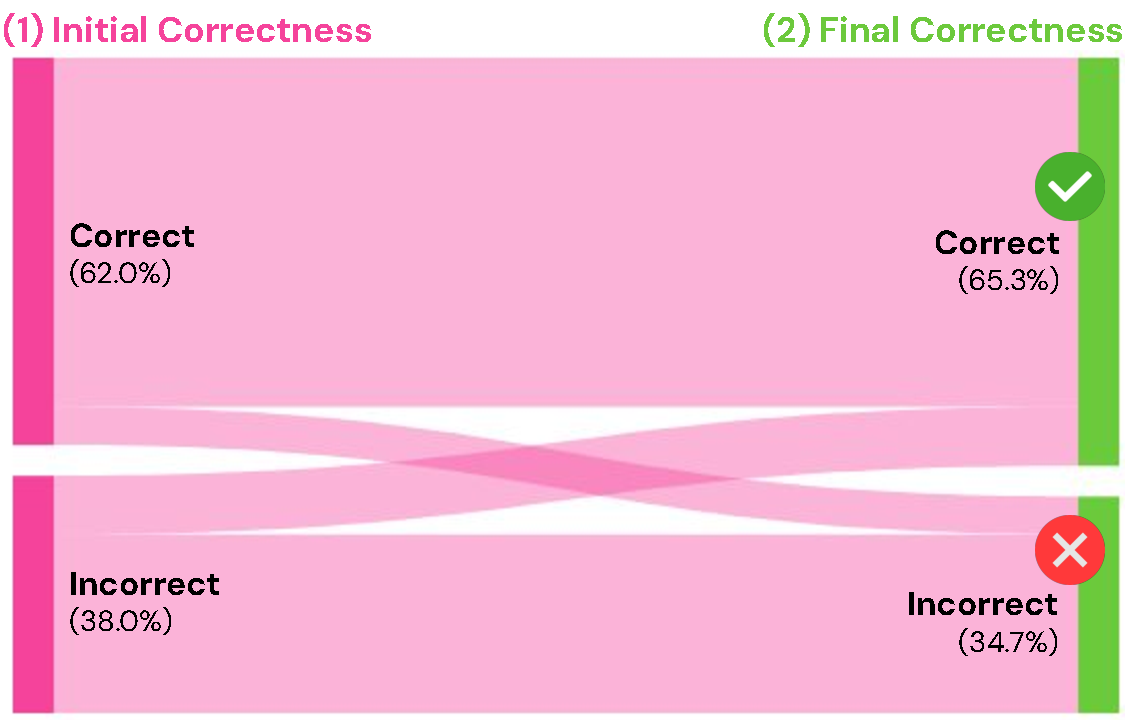
\includegraphics[width=0.31\textwidth]{figure/self-reflect.pdf}} 
    \subfigure[Debate-Only]{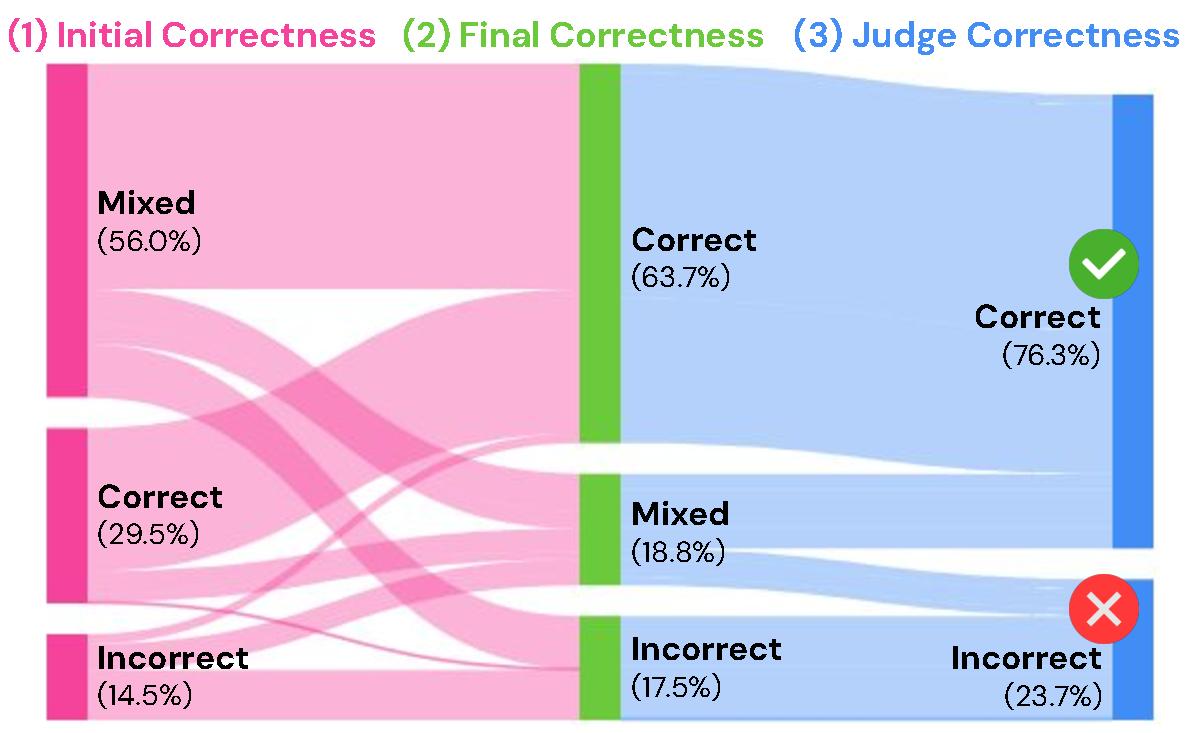
\includegraphics[width=0.33\textwidth]{figure/multi_r.pdf}} 
    \subfigure[Self-Reflect+Debate]{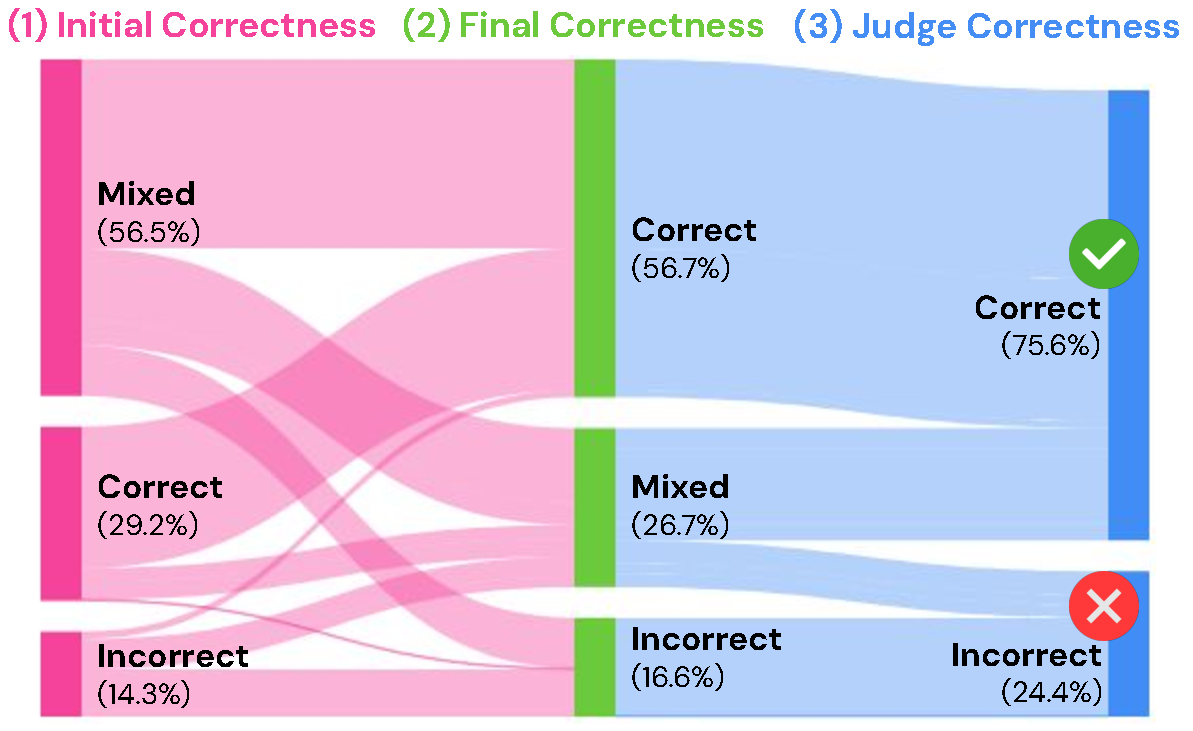
\includegraphics[width=0.33\textwidth]{figure/selective_r.pdf}} 
    
    \caption{How model decisions evolve through (a) Self-Reflection, (b) Debate-Only, and (c) Self-Reflect+Debate, each aggregated across all LLMs or LLM combinations. 
    \textbf{\textcolor{darkpurple}{1) Initial Correctness}}: whether the model's initial decision is correct; \textbf{\textcolor{darkgreen}{2) Final Correctness}}: whether the individual model's final decision is correct; \textbf{\textcolor{bblue}{3) Judge Correctness}}: whether the judge LLM's debate adjudication decision is correct. If both models evaluated in  \textbf{\textcolor{darkgreen}{2}} agree, this is determined by the correctness of the agreed-upon answer. For (b) and (c), ``Correct'' indicates both models' decisions are correct, ``Incorrect'' as both incorrect, and ``Mixed'' as when the two models generate differing decisions (\textit{e.g.,} one correct and one wrong). Detailed results per LLM or LLM combination are in Appendix \ref{appendix:detailed_dynamics}.}
    \label{fig:sankey_chart}
\end{figure*}

% \textbf{\textcolor{bblue}{(2) Behavioral dynamic}:} whether the model changes its decision;


\subsection{Result Summary}

Overall, these results show that multi-agent debate enables smaller LLMs to achieve performance comparable to the much larger judge LLM, \textsc{Gemma-2-27b} (79.2\%). Our best 7-9B single model baseline lag behind that larger model by 8.5 points (\textsc{Yi-1.5} with rule-of-thumb information (70.7\%)). Multi-agent debate narrows, and, in some cases, closes this gap: among the individual debate accuracies (\textcolor{rred}{\textbf{D($\mathcal{M}_i$)}}, \textcolor{purple}{\textbf{S+D($\mathcal{M}_i$)}}), the best performance is attained with \textsc{Gemma-2} and \textsc{EXAONE-3} in the Self-Reflect+Debate setup, with \textsc{Gemma-2} achieving a mean accuracy of 79.6\%. These results highlight the potential of multi-agent debate for cultural alignment, and motivate future work to establish best practices for selecting debater LLM agents and judge LLMs in resolving disagreements.

% \mc{Is the difference between 80.1 and 81.5 statistically significant? if not it does not exceed, it matches the performance; also it is perhaps worth pointing out what is the best result we can get without a large LLM judge and how it compares to the GEMMA-27b performance: can we approach the performance of a much larger model with smaller models? Among the models tested, with single models we can get about 10 points below (Yi-1.5) but with debate we can get much closer (I think best of D(M1), D(M2), S+D(M1) and S+D(M2) scores is 79.5?)}

% \mc{I am missing an overall recommendation about what is a good strategy, given that results vary across the specific LLMs used. For a new related task, given these rsults, how should I go about picking LLMs and how to use them? Or do we not have enoiugh informatino to provide recommenations yet, and the recommendation is simply to explore multi-agent debate and that future work is needed to establish best practices for selecting debate participants and resolving disagreements?}

% \zk{I think there is winning strategy for coming up with a final decision.. I think the main takeaway from the multi-debate agent is that we can reach larger llm performance with debating 2 smaller llms + debate-only show better individual debate accuracies + self-reflect+debate benefits more from the judge LLM, leading up to higher mean accuracy}
